\documentclass[lettersize,journal]{IEEEtran}
\usepackage{amsmath,amsfonts}
\usepackage{algorithmic}
\usepackage{algorithm}
\usepackage{array}
\usepackage[caption=false,font=normalsize,labelfont=sf,textfont=sf]{subfig}
\usepackage{textcomp}
\usepackage{stfloats}
\usepackage{url}
\usepackage{verbatim}
\usepackage{graphicx}
\usepackage{cite}
\usepackage{amssymb}
\usepackage{nicefrac}
\usepackage{booktabs}  % Para líneas mejoradas en tablas
\usepackage{multirow}  % Para combinar filas si es necesario
\usepackage{tikz}      % Para dibujar los triángulos
\usepackage{subcaption}   % Para las subfiguras

\hyphenation{op-tical net-works semi-conduc-tor IEEE-Xplore}
% updated with editorial comments 8/9/2021

\begin{document}

\title{Instrumental Odour Monitoring System Optimized for Drone Applications}

\author{\IEEEauthorblockN{Javier Alonso-Valdesueiro\IEEEauthorrefmark{1}\IEEEauthorrefmark{2},
Santiago Marco-Colás\IEEEauthorrefmark{1}\IEEEauthorrefmark{2} and Agustín Gutiérrez-Gálvez\IEEEauthorrefmark{1}\IEEEauthorrefmark{2}}
\\
\IEEEauthorblockA{
\IEEEauthorrefmark{1} Department of Electronic and Biomedical Engineering, University of Barcelona,
\\
\IEEEauthorrefmark{2} Signal and Information Processing for Sensing Systems, Institute for Bioengineering of Catalunya}



        % <-this % stops a space
\thanks{This contribution has been funded from ATTRACT, a European Union Horizon 2020 research and innovation project, under grant agreement No. 101004462. The research has been also partially funded by IBEC-CERCA consortium and Generalitat de Catalunya (expedient 2021 SGR 01393).}

\thanks{Manuscript received April 19, 2021; revised August 16, 2021.}}

% The paper headers
\markboth{IEEE Transactions on Instrumentation and Measurement,~Vol.~XX, No.~X, December~2055}%
{Shell \MakeLowercase{\textit{et al.}}: A Sample Article Using IEEEtran.cls for IEEE Journals}

\IEEEpubid{0000--0000/00\$00.00~\copyright~20255 IEEE}
% Remember, if you use this you must call \IEEEpubidadjcol in the second
% column for its text to clear the IEEEpubid mark.

\maketitle

\begin{abstract}
In this contribution, a novel design for an Instrumental Odour Monitoring System (IOMS) is presented. This evolution of the IOMS concept is designed to be mounted on a drone, enabling the generation of 3D maps of gas concentrations and odour levels during flight. It features fast-response gas chambers, a rapid data acquisition architecture, a modular design, and fast GPS RTK tracking. The performance of this innovative design has been tested under controlled conditions, comparing its performance with existing designs. The results show that the time for the gas concentration inside the IOMS to reach the limit of detection of the sensors is approximately 3-7 seconds faster than that observed in traditional IOMS designs. Additionally, measurements taken during test flights with a conventional IOMS are compared with those obtained using the new design. In every flight, the new IOMS produces results tenths of seconds faster than the conventional designs. These results, both in the laboratory and in the field, indicate that the modifications in the new IOMS design enable it to respond rapidly to changes caused by the drone's swift movements. This fast response and rapid tracking make the novel design more suitable for fast 3D map of gas concentrations and odour levelthan conventional IOMS designs.  
\end{abstract}

\begin{IEEEkeywords}
IOMS; Drone-based odour monitoring; 3D odour mapping; Gas concentration mapping; Fast-response gas chambers; Electronic nose; Malodours; Machine learning; Odour intensity prediction
\end{IEEEkeywords}

\section{Introduction}
\label{sec:intro}
\IEEEPARstart{I}{nstrumental} Odour Monitoring Systems (IOMS) have been deployed in Wastewater Treatment Plants (WWTPs) over the past decade \cite{persaud2005medical, capelli2014electronic, di2017real, blanco2018development}. These systems are used for odour quantification and monitoring due to their effectiveness in measuring gases such as H$_2$S, NH$_3$, and others producing malodorous \cite{cangialosi2018, daelman2012methane}. Consequently, in recent years, they have become commercial products and are being installed at WWTP fences and critical points across Europe \cite{blanco2018development, prudenza2023implementation, cipriano2019evolution, deshmukh2015application}. However, these deployments are time-consuming, requiring extensive and costly calibration procedures. Furthermore, they lack flexibility in case of plant changes and cannot produce a comprehensive map of the plant unless multiple IOMS units are deployed around and inside the facility \cite{ratti2024real}.

In recent years, drone-based IOMS have emerged for rapid gas concentration characterization and odour mapping in the industrial landscape \cite{pobkrut2016sensor, burgues2021rhinos, burgues2022characterization}. Their applications include methane leak control \cite{tassielli2024detection}, fire detection with source location \cite{yandouzi2023investigation}, and air quality monitoring \cite{burgués2023drone}. In particular, studies on WWTPs have shown that these systems can produce 3D maps of gas concentration results much faster than commercial IOMS for the entire plant \cite{burgués2019high}, enabling data scientists to develop odour quantification models \cite{cangialosi2022integrating, benegiamo2024optimization}.

Despite these results, experience has shown that drone-mounted designs struggle to follow rapid variations of its surrounding air \cite{burgues2021rhinos, burgues2022characterization, benegiamo2024optimization}. Consequently, the drone's speed (typically $\sim$$10$~\nicefrac{m}{s}) when moving around the plant for 3D mapping is limited by the response time of the measuring system. Also, windy conditions produce plumes of odour and the conventional IOMSs struggle to work in these conditions (wind speed $\leq 10$~\nicefrac{km}{h}). This limitation reduces the applicability of IOMSs to quantify static sources and operate in favorable conditions.

Recent studies have shown that a careful design of the gas chambers containing the sensors in an IOMS significantly reduces the time needed to reach the sensors' limit of detection \cite{valdesueiro24dronE}. This reduction in response time impacts on the requirements of sensor data and GPS location data acquisition architectures of the IOMS. Consequently, the traditional IOMS design, even in its drone-mounted version \cite{burgues2021rhinos}, requires a substantial review.

This work presents the mentioned review of the conventional IOMS design, featuring a very fast response time, rapid data acquisition architecture, and centimeter-precise RTK GPS location. This platform is capable of tracking rapid changes in the surrounding air, addressing the limitations of conventional IOMSs when mounted on drones (such as drone speed and windy weather conditions). During laboratory tests, the novel design has shown faster response (in the tenths of seconds) to an odorous step than a conventional IOMS and fast plume tracking. This behavior has been confirmed during test flights (at UPC facilities droneLab, Castelldefels, Spain). 

Therefore, this contribution is organized as follows: Section \ref{sec:IOMS} provides a description of the novel IOMS, including its gas chambers, data acquisition architecture, communications, and GPS data management. Section \ref{sec:labChar} presents a comprehensive performance characterization of the IOMS by comparing its response in various experiments with that of a conventional design. Section \ref{sec:flyPerf} summarizes the flying tests assessing the IOMS performance. Finally, Section \ref{sec:conclusions} summarizes the achievements of this design, outlining the potential applications of this optimized IOMS.
\IEEEpubidadjcol
 
\section{IOMS Description}
\label{sec:IOMS}

\begin{figure*}[t] % t para colocar la figura en la parte superior
	\centering
	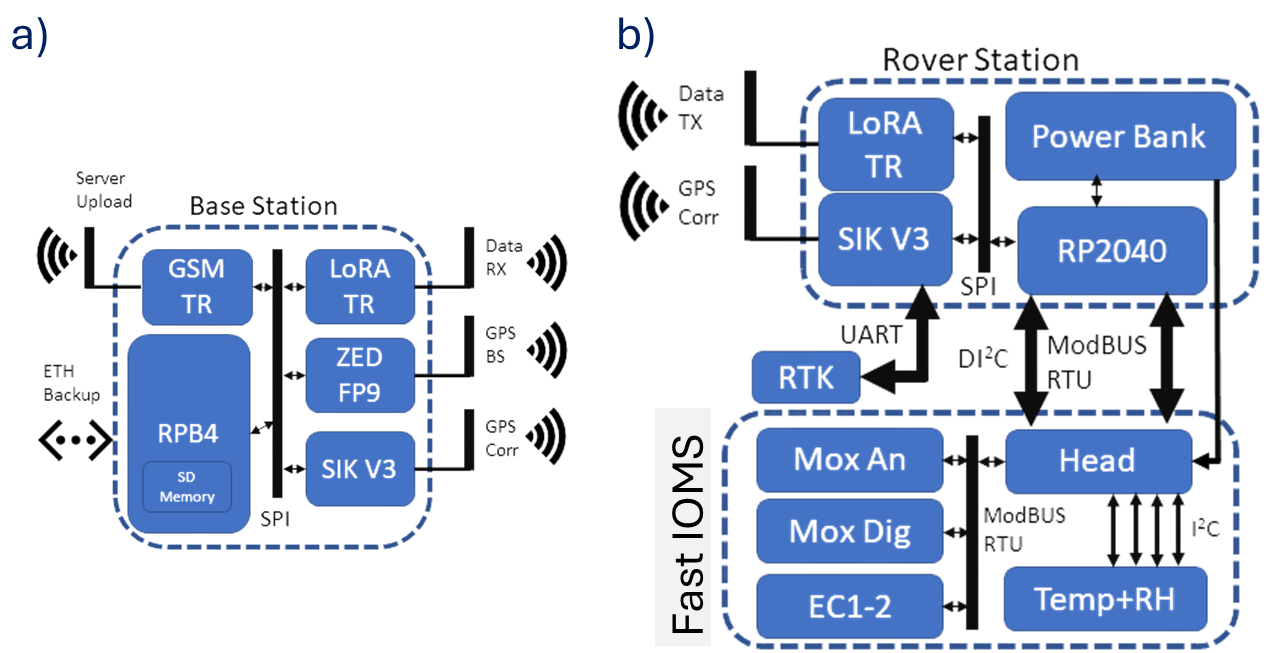
\includegraphics[width=0.53\linewidth]{./images/fig1_ab.png}
	\hfill
	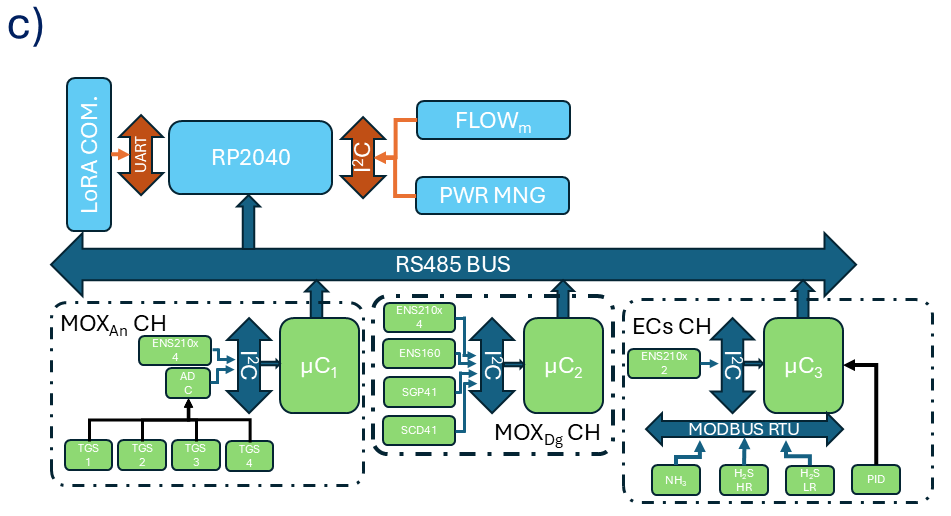
\includegraphics[width=0.45\linewidth]{./images/fig1_c.png}
	\hfill
	\caption{Graphical description of the Instrumental Odour Monitoring System. a) Block diagram of the Base Station (BS). It is based on a Raspberry pi 4B+ and communicates with the mobile part of the IOMS via Peer two Peer LoRA connection. It also provide GPS data to the RTK GPS module for corrections and communicates with an external server via GSM router. b) Block diagram of the mobile part of the IOMS. The Rover Station (RS) is placed on the drone and it controls the power consumption and gets data from the FastIOMS system. This system provides data from three chambers, each with different sensors inside, air flow coming inside the the chambers and temperature and relative humidity of the air in contact with each sensor.}
	\label{fig:iomsDescp}
\end{figure*}

Figures~\ref{fig:iomsDescp}~(a), (b) and (c) show the architecture of the novel IOMS. The system is divided in two parts. The mobile part contains the Rover Station (RS), the RTK GPS system, the Bag Sampler (BSplr), and the Fast IOMS (see figure~\ref{fig:iomsPhoto}). The ground based system (Base Station or BS) is placed near by the fliying area for monitoring, logging and control duties.

The RS is placed on the drone and it controls the power consumption, gets data from the Fast-IOMS system, and controls the activation of the BSplr. The Fast-IOMS system provides data from three chambers, each with different sensors inside, air flow coming inside the the chambers and temperature and relative humidity of the air in contact with each sensor. This data is sent via Peer-to-Peer LoRA communication to the BS. At the BS, the data is plotted for information of the operator, logged in a hardrive and sent to an external server for further analysis. The BS connects with the external server via a GSM router.

At the same time the data from the Fast-IOMS is logged, data with centimeter precission is added to the generated files. This data is provided by the RTK GPS module once the module recives GPS location from the BS and makes its corrections. The module is based on a ZED-F9P module from U-Blox.

Finally, whenever the operator decides to activate the BSplr, the BS sends a command to the RS via LoRA to activate the Bag Sampler. This system is based on a small pump that sucks air from the environment and stores it in a bag for further analysis.

\begin{figure}[!t] % t para colocar la figura en la parte superior
	\centering
	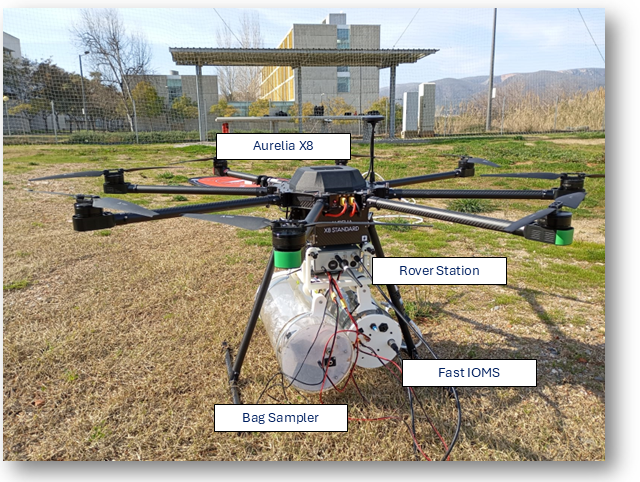
\includegraphics[width=1\linewidth]{./images/fig3.png}
	\hfill
	\caption{Novel IOMS mounted on the drone with the Bag Sampler. The Rover Station is placed close to the drone chassis for protection. The Fast IOMS and Bag Sampler air inlets are connected two both 10 meters PTFE tubes.}
	\label{fig:iomsPhoto}
\end{figure}

\subsection{Fast IOMS}
\label{ssec:fastIOMS}
The Fast-IOMS consists of 4 chambers with 3 electrochemical sensors, one Photo Ionization Detector (PID), and MOx sensors from different manufacturers. Table 1 summarizes the sensors placed inside the chambers.
Every chamber has its own microcontroller ($\mu$C) SAMD21 for acquiring and transmitting the data. Each has a hardware interrupt line that activates the communication protocol via RS$485$. The $\mu$Cs also have a USB-C port for debugging and stand-alone functionality.

The MoxAn chamber consists of 4 small cavities ($0.6$~cm$^{3}$) accommodating 4 TGS MOx sensors from Figaro. Currently, the sensors (TGS$2600$, TGS$2602$, TGS$2611$, and TGS$2620$) operate with the same PWM signal applied to their heater resistance. Voltage is acquired using an ADS$1115$ ADC connected to the $\mu$C via I$^{2}$C. Table~\ref{tab:fastIOMSsensors} summarizes the sensors placed inside each chamber.


Temperature and relative humidity inside each cavity are sampled by ENS$210$ sensors from Sensirion. The resistance of the $4$ MOx sensors is sent to the RS via RS$485$ at a maximum rate of $10$ Hz, along with the data from the ENS$210$ sensors, sampled every second.
With a similar design, the MoxDig chamber consists of 4 small cavities where $3$ digital MOx sensors and one photoacoustic sensor are placed. The SGP$41$, the ENS$160$, and the BM$688$ are configured in their single-shot acquisition mode. The SCD$41$ is configured in its periodic sampling mode.
As in the MoxAn chamber, 4 ENS$210$ sensors are placed inside for temperature and relative humidity monitoring. 

The other two chambers host $3$ electrochemical sensors from Membrapor and a Photoionization Detector (PID) from Alphasense. The H$_{2}$S sensors are placed together in the same chamber with an additional ENS210 sensor monitoring temperature and relative humidity inside. The NH$_{3}$ sensor is placed in the second chamber with the PID, also with an additional ENS$210$ sensor. The electrochemical sensors are controlled by a PCB from Membrapor and the voltage produced by the PID is acquired using an ADS$1115$ ADC. 

The raw data from the three  are sent to the RS at a maximum rate of $1$~$\nicefrac{Hz}{sensor}$ along with their corresponding temperature and relative humidity data from the ENS$210$ sensors (sampled every $6$ seconds).

\begin{table}
	\caption{Summary of the sensors placed inside each chamber and their main characteristics.}
	\setlength{\tabcolsep}{0.5\tabcolsep}% Shrink \tabcolsep by 30%
	\centering
	\begin{tabular}{ *{4}{c} }
	\toprule
	\multirow{2}{*}{\textbf{Chamber}} & & \textbf{Chamber Characteristics}\\
		& \textit{Sensors} & \textit{Chamber} & \textit{Number of}\\
		& {Included} & \textit{Volume} & \textit{ENS$210$}\\
		& &\textit{(cm$^{3}$)} & \textit{($^{\circ}$, RH($\%$))}\\
		\midrule
		MoxAn & TGS2600, TGS2602,   & 0.6    & 4\\
		    & TGS2611, TGS2620	  &        &  \\
		MoxDig & SGP41, ENS160, & 0.6    & 4\\
		     & BM688, SCD41	  &        &  \\
		ECS & H2S/C-50, & 4 & 1\\
		  & H2S/C-200 & & \\
		ECs+PID & NH3/C-100, PID & 4 & 1\\
		\bottomrule
	\end{tabular}
	\label{tab:fastIOMSsensors}
\end{table}
 
 
The Fast-IOMS also hosts a pump connected upstream of the fluidic path. It can provide $3.5$~slm of air mass flow when every chamber is connected to it. A flow meter (FS$2012$ from Renesas) has been placed at the entrance of the chambers to monitor the air entering the Fast-IOMS. This data is sent directly to the RS via differential I2C.

\subsection{Rover Station}
\label{ssec:roverStation}

As it is shown in figure~\ref{fig:iomsPhoto}, the RS is comfortably attached to the lower belly of the AAurelia X8 octocopter. Ther RS is based on a two core RP2040 $\mu$C which controls the power consumption of the Flying system (Fast-IOMS and itself) via I$^{2}$C. It si connected to the Fast-IMS via a RS$485$ bus (as depicted in figure~\ref{fig:iomsDescp}~(c)) and produces bursts of data every $2$ seconds. Each burst of data corresponds to one chamber and contains $6$ different measurments of every sensor stamped with the corresponding temperature and Relative humidity data.

Each data burst is packed and sent to the BS via Peer-to-Peer LoRA communication. The LoRA module is controlled via a Serial-UART bus (see figure~\ref{fig:iomsDescp}~(c)) and works at $915$~MHz sending packets of $256$ bytes.

\subsection{Base Station}
\label{ssec:baseStation}

The BS is based on a Raspberry pi 4B+ and communicates with the mobile part of the IOMS via Peer two Peer LoRA connection as explained in the previous section. As the data is comming, it is plotted by a Python-based Graphical User Interface (GUI) which is running continouslly. The GUI also allows to control the bag sampler activation sending via LoRA commands to the RS. This GUI also logs the data in a hardrive and sends the created files to a FTTP server via a GSM router.

\subsection{RTK GPS}
\label{ssec:rtkGPS}
In paralel to the transmission of the data from the RS to the BS, the RTK GPS module (ZED-F9P from U-Blox) is receiving GPS data from the BS (generated by another ZED-F9P module) and making corrections to the GPS location. This data is sent to the BS via Peer-to-Peer connection at $433$~MHz and is logged in the same file as the data from the Fast-IOMS. 

\section{IOMS Performance Characterization}
\label{sec:labChar}

\begin{figure*}[t] % t para colocar la figura en la parte superior
	\centering
	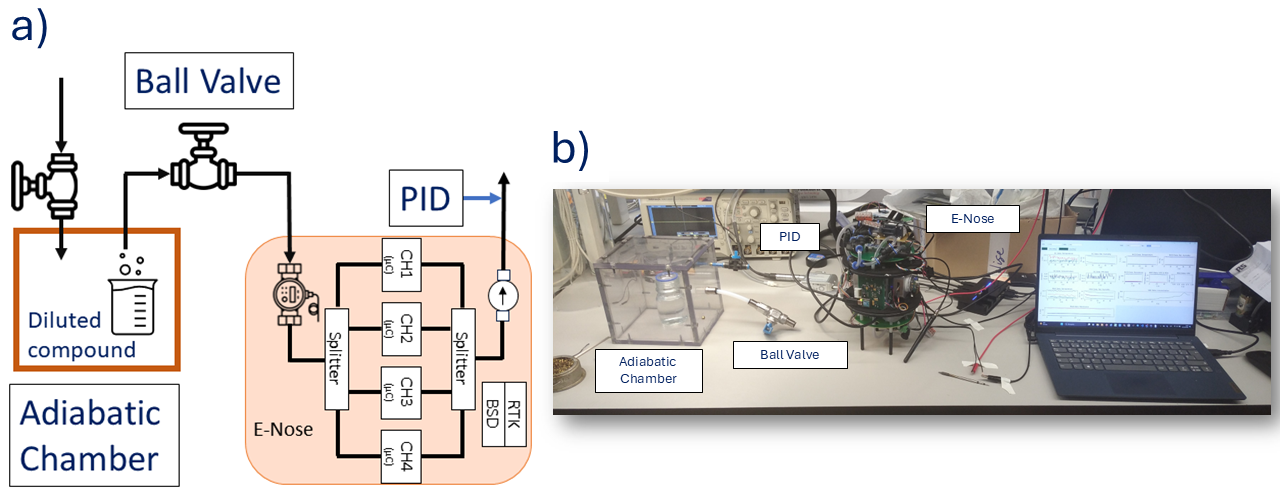
\includegraphics[width=0.53\linewidth]{./images/fig2_ab.png}
	\hfill
	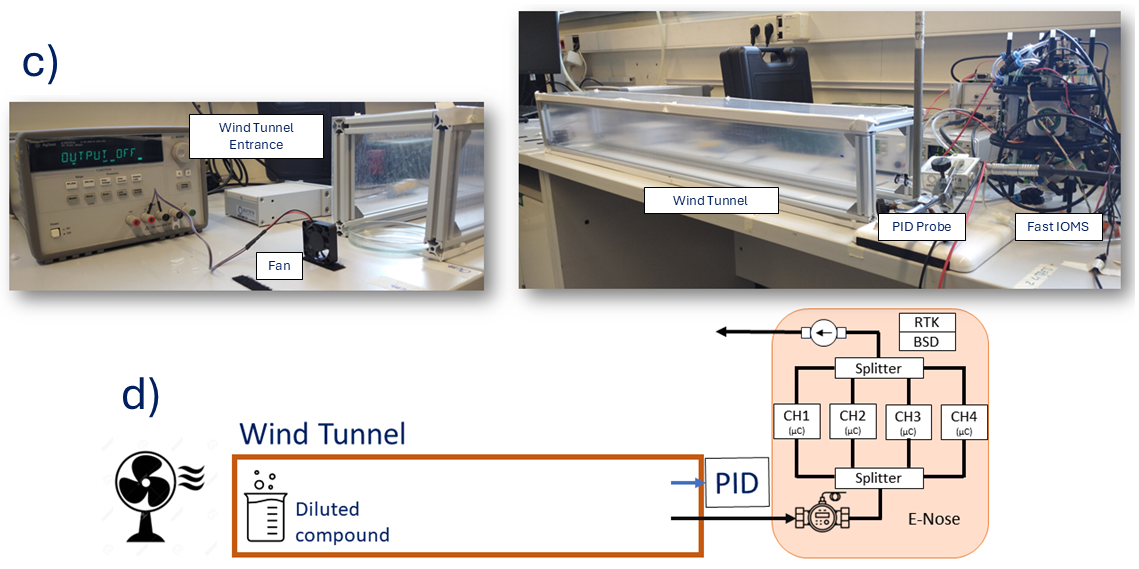
\includegraphics[width=0.45\linewidth]{./images/fig2_cd.png}
	\hfill
	\caption{Experimental setups used for characterizing the Fast IOMS system at the laboratory. a) First setup: the fast IOMS is connected to ball valve acting as a exhaust valve of an adiabatic chamber. The diluted compound is placed inside the chamber and leaved there for 5 minutes with the inlet valve and the exhaust valve closed. After 5 minutes both valves are open and the Fast IOMS inlet is connected to the exhaust valve for data logging. b) Practical realization of the first experimental setup. c) Second setup: The Fast IOMS inlet is placed alongside the probe tip of a 201B miniPID from AURORA Inc. at the end of a wind tunnel. At the entrance of the wind tunnel, a small petri dish with 25mL of the diluted compound with a small fan is placed. The fan is turned on and off in 20 seconds intervals. d) Practical realization of the second setup.}
	\label{fig:characSetups}
\end{figure*}

\begin{list}{}{}
\item{\url{http://www.latex-community.org/}} 
\item{\url{https://tex.stackexchange.com/} }
\end{list}

\section{Drone-mounted IOMS and Flight Performance}
\label{sec:flyPerf}
See \cite{ref1,ref2,ref3,ref4,ref5} for resources on formatting math into text and additional help in working with \LaTeX .

\section{Conclusions}
\label{sec:conclusions}
For some of the remainer of this sample we will use dummy text to fill out paragraphs rather than use live text that may violate a copyright.

Itam, que ipiti sum dem velit la sum et dionet quatibus apitet voloritet audam, qui aliciant voloreicid quaspe volorem ut maximusandit faccum conemporerum aut ellatur, nobis arcimus.
Fugit odi ut pliquia incitium latum que cusapere perit molupta eaquaeria quod ut optatem poreiur? Quiaerr ovitior suntiant litio bearciur?

Onseque sequaes rectur autate minullore nusae nestiberum, sum voluptatio. Et ratem sequiam quaspername nos rem repudandae volum consequis nos eium aut as molupta tectum ulparumquam ut maximillesti consequas quas inctia cum volectinusa porrum unt eius cusaest exeritatur? Nias es enist fugit pa vollum reium essusam nist et pa aceaqui quo elibusdandis deligendus que nullaci lloreri bla que sa coreriam explacc atiumquos simolorpore, non prehendunt lam que occum\cite{ref6} si aut aut maximus eliaeruntia dia sequiamenime natem sendae ipidemp orehend uciisi omnienetus most verum, ommolendi omnimus, est, veni aut ipsa volendelist mo conserum volores estisciis recessi nveles ut poressitatur sitiis ex endi diti volum dolupta aut aut odi as eatquo cullabo remquis toreptum et des accus dolende pores sequas dolores tinust quas expel moditae ne sum quiatis nis endipie nihilis etum fugiae audi dia quiasit quibus.
\IEEEpubidadjcol
Ibus el et quatemo luptatque doluptaest et pe volent rem ipidusa eribus utem venimolorae dera qui acea quam etur aceruptat.
Gias anis doluptaspic tem et aliquis alique inctiuntiur?

Sedigent, si aligend elibuscid ut et ium volo tem eictore pellore ritatus ut ut ullatus in con con pere nos ab ium di tem aliqui od magnit repta volectur suntio. Nam isquiante doluptis essit, ut eos suntionsecto debitiur sum ea ipitiis adipit, oditiore, a dolorerempos aut harum ius, atquat.

Rum rem ditinti sciendunti volupiciendi sequiae nonsect oreniatur, volores sition ressimil inus solut ea volum harumqui to see\eqref{deqn_ex1a} mint aut quat eos explis ad quodi debis deliqui aspel earcius.

\begin{equation}
\label{deqn_ex1a}
x = \sum_{i=0}^{n} 2{i} Q.
\end{equation}

Alis nime volorempera perferi sitio denim repudae pre ducilit atatet volecte ssimillorae dolore, ut pel ipsa nonsequiam in re nus maiost et que dolor sunt eturita tibusanis eatent a aut et dio blaudit reptibu scipitem liquia consequodi od unto ipsae. Et enitia vel et experferum quiat harum sa net faccae dolut voloria nem. Bus ut labo. Ita eum repraer rovitia samendit aut et volupta tecupti busant omni quiae porro que nossimodic temquis anto blacita conse nis am, que ereperum eumquam quaescil imenisci quae magnimos recus ilibeaque cum etum iliate prae parumquatemo blaceaquiam quundia dit apienditem rerit re eici quaes eos sinvers pelecabo. Namendignis as exerupit aut magnim ium illabor roratecte plic tem res apiscipsam et vernat untur a deliquaest que non cus eat ea dolupiducim fugiam volum hil ius dolo eaquis sitis aut landesto quo corerest et auditaquas ditae voloribus, qui optaspis exero cusa am, ut plibus.


\section{Some Common Elements}
\subsection{Sections and Subsections}
Enumeration of section headings is desirable, but not required. When numbered, please be consistent throughout the article, that is, all headings and all levels of section headings in the article should be enumerated. Primary headings are designated with Roman numerals, secondary with capital letters, tertiary with Arabic numbers; and quaternary with lowercase letters. Reference and Acknowledgment headings are unlike all other section headings in text. They are never enumerated. They are simply primary headings without labels, regardless of whether the other headings in the article are enumerated. 

\subsection{Citations to the Bibliography}
The coding for the citations is made with the \LaTeX\ $\backslash${\tt{cite}} command. 
This will display as: see \cite{ref1}.

For multiple citations code as follows: {\tt{$\backslash$cite\{ref1,ref2,ref3\}}}
 which will produce \cite{ref1,ref2,ref3}. For reference ranges that are not consecutive code as {\tt{$\backslash$cite\{ref1,ref2,ref3,ref9\}}} which will produce  \cite{ref1,ref2,ref3,ref9}

\subsection{Lists}
In this section, we will consider three types of lists: simple unnumbered, numbered, and bulleted. There have been many options added to IEEEtran to enhance the creation of lists. If your lists are more complex than those shown below, please refer to the original ``IEEEtran\_HOWTO.pdf'' for additional options.\\

\subsubsection*{\bf A plain  unnumbered list}
\begin{list}{}{}
\item{bare\_jrnl.tex}
\item{bare\_conf.tex}
\item{bare\_jrnl\_compsoc.tex}
\item{bare\_conf\_compsoc.tex}
\item{bare\_jrnl\_comsoc.tex}
\end{list}

\subsubsection*{\bf A simple numbered list}
\begin{enumerate}
\item{bare\_jrnl.tex}
\item{bare\_conf.tex}
\item{bare\_jrnl\_compsoc.tex}
\item{bare\_conf\_compsoc.tex}
\item{bare\_jrnl\_comsoc.tex}
\end{enumerate}

\subsubsection*{\bf A simple bulleted list}
\begin{itemize}
\item{bare\_jrnl.tex}
\item{bare\_conf.tex}
\item{bare\_jrnl\_compsoc.tex}
\item{bare\_conf\_compsoc.tex}
\item{bare\_jrnl\_comsoc.tex}
\end{itemize}





\subsection{Figures}
Fig. 1 is an example of a floating figure using the graphicx package.
 Note that $\backslash${\tt{label}} must occur AFTER (or within) $\backslash${\tt{caption}}.
 For figures, $\backslash${\tt{caption}} should occur after the $\backslash${\tt{includegraphics}}.

\begin{figure}[!t]
\centering
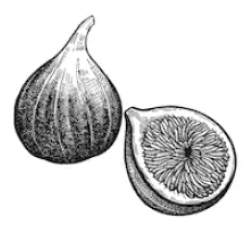
\includegraphics[width=2.5in]{fig1}
\caption{Simulation results for the network.}
\label{fig_1}
\end{figure}

Fig. 2(a) and 2(b) is an example of a double column floating figure using two subfigures.
 (The subfig.sty package must be loaded for this to work.)
 The subfigure $\backslash${\tt{label}} commands are set within each subfloat command,
 and the $\backslash${\tt{label}} for the overall figure must come after $\backslash${\tt{caption}}.
 $\backslash${\tt{hfil}} is used as a separator to get equal spacing.
 The combined width of all the parts of the figure should do not exceed the text width or a line break will occur.
%
\begin{figure*}[!t]
\centering
\subfloat[]{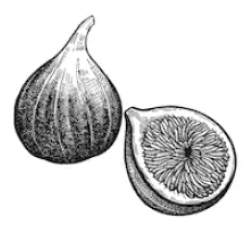
\includegraphics[width=2.5in]{fig1}%
\label{fig_first_case}}
\hfil
\subfloat[]{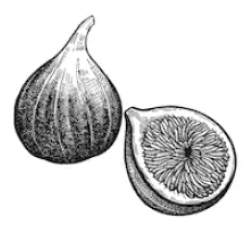
\includegraphics[width=2.5in]{fig1}%
\label{fig_second_case}}
\caption{Dae. Ad quatur autat ut porepel itemoles dolor autem fuga. Bus quia con nessunti as remo di quatus non perum que nimus. (a) Case I. (b) Case II.}
\label{fig_sim}
\end{figure*}

Note that often IEEE papers with multi-part figures do not place the labels within the image itself (using the optional argument to $\backslash${\tt{subfloat}}[]), but instead will
 reference/describe all of them (a), (b), etc., within the main caption.
 Be aware that for subfig.sty to generate the (a), (b), etc., subfigure
 labels, the optional argument to $\backslash${\tt{subfloat}} must be present. If a
 subcaption is not desired, leave its contents blank,
 e.g.,$\backslash${\tt{subfloat}}[].


 

\section{Tables}
Note that, for IEEE-style tables, the
 $\backslash${\tt{caption}} command should come BEFORE the table. Table captions use title case. Articles (a, an, the), coordinating conjunctions (and, but, for, or, nor), and most short prepositions are lowercase unless they are the first or last word. Table text will default to $\backslash${\tt{footnotesize}} as
 the IEEE normally uses this smaller font for tables.
 The $\backslash${\tt{label}} must come after $\backslash${\tt{caption}} as always.
 
\begin{table}[!t]
\caption{An Example of a Table\label{tab:table1}}
\centering
\begin{tabular}{|c||c|}
\hline
One & Two\\
\hline
Three & Four\\
\hline
\end{tabular}
\end{table}

\section{Algorithms}
Algorithms should be numbered and include a short title. They are set off from the text with rules above and below the title and after the last line.

\begin{algorithm}[H]
\caption{Weighted Tanimoto ELM.}\label{alg:alg1}
\begin{algorithmic}
\STATE 
\STATE {\textsc{TRAIN}}$(\mathbf{X} \mathbf{T})$
\STATE \hspace{0.5cm}$ \textbf{select randomly } W \subset \mathbf{X}  $
\STATE \hspace{0.5cm}$ N_\mathbf{t} \gets | \{ i : \mathbf{t}_i = \mathbf{t} \} | $ \textbf{ for } $ \mathbf{t}= -1,+1 $
\STATE \hspace{0.5cm}$ B_i \gets \sqrt{ \textsc{max}(N_{-1},N_{+1}) / N_{\mathbf{t}_i} } $ \textbf{ for } $ i = 1,...,N $
\STATE \hspace{0.5cm}$ \hat{\mathbf{H}} \gets  B \cdot (\mathbf{X}^T\textbf{W})/( \mathbb{1}\mathbf{X} + \mathbb{1}\textbf{W} - \mathbf{X}^T\textbf{W} ) $
\STATE \hspace{0.5cm}$ \beta \gets \left ( I/C + \hat{\mathbf{H}}^T\hat{\mathbf{H}} \right )^{-1}(\hat{\mathbf{H}}^T B\cdot \mathbf{T})  $
\STATE \hspace{0.5cm}\textbf{return}  $\textbf{W},  \beta $
\STATE 
\STATE {\textsc{PREDICT}}$(\mathbf{X} )$
\STATE \hspace{0.5cm}$ \mathbf{H} \gets  (\mathbf{X}^T\textbf{W} )/( \mathbb{1}\mathbf{X}  + \mathbb{1}\textbf{W}- \mathbf{X}^T\textbf{W}  ) $
\STATE \hspace{0.5cm}\textbf{return}  $\textsc{sign}( \mathbf{H} \beta )$
\end{algorithmic}
\label{alg1}
\end{algorithm}

Que sunt eum lam eos si dic to estist, culluptium quid qui nestrum nobis reiumquiatur minimus minctem. Ro moluptat fuga. Itatquiam ut laborpo rersped exceres vollandi repudaerem. Ulparci sunt, qui doluptaquis sumquia ndestiu sapient iorepella sunti veribus. Ro moluptat fuga. Itatquiam ut laborpo rersped exceres vollandi repudaerem. 
\section{Mathematical Typography \\ and Why It Matters}

Typographical conventions for mathematical formulas have been developed to {\bf provide uniformity and clarity of presentation across mathematical texts}. This enables the readers of those texts to both understand the author's ideas and to grasp new concepts quickly. While software such as \LaTeX \ and MathType\textsuperscript{\textregistered} can produce aesthetically pleasing math when used properly, it is also very easy to misuse the software, potentially resulting in incorrect math display.

IEEE aims to provide authors with the proper guidance on mathematical typesetting style and assist them in writing the best possible article. As such, IEEE has assembled a set of examples of good and bad mathematical typesetting \cite{ref1,ref2,ref3,ref4,ref5}. 

Further examples can be found at \url{http://journals.ieeeauthorcenter.ieee.org/wp-content/uploads/sites/7/IEEE-Math-Typesetting-Guide-for-LaTeX-Users.pdf}

\subsection{Display Equations}
The simple display equation example shown below uses the ``equation'' environment. To number the equations, use the $\backslash${\tt{label}} macro to create an identifier for the equation. LaTeX will automatically number the equation for you.
\begin{equation}
\label{deqn_ex1}
x = \sum_{i=0}^{n} 2{i} Q.
\end{equation}

\noindent is coded as follows:
\begin{verbatim}
\begin{equation}
\label{deqn_ex1}
x = \sum_{i=0}^{n} 2{i} Q.
\end{equation}
\end{verbatim}

To reference this equation in the text use the $\backslash${\tt{ref}} macro. 
Please see (\ref{deqn_ex1})\\
\noindent is coded as follows:
\begin{verbatim}
Please see (\ref{deqn_ex1})\end{verbatim}

\subsection{Equation Numbering}
{\bf{Consecutive Numbering:}} Equations within an article are numbered consecutively from the beginning of the
article to the end, i.e., (1), (2), (3), (4), (5), etc. Do not use roman numerals or section numbers for equation numbering.

\noindent {\bf{Appendix Equations:}} The continuation of consecutively numbered equations is best in the Appendix, but numbering
 as (A1), (A2), etc., is permissible.\\

\noindent {\bf{Hyphens and Periods}}: Hyphens and periods should not be used in equation numbers, i.e., use (1a) rather than
(1-a) and (2a) rather than (2.a) for subequations. This should be consistent throughout the article.

\subsection{Multi-Line Equations and Alignment}
Here we show several examples of multi-line equations and proper alignments.

\noindent {\bf{A single equation that must break over multiple lines due to length with no specific alignment.}}
\begin{multline}
\text{The first line of this example}\\
\text{The second line of this example}\\
\text{The third line of this example}
\end{multline}

\noindent is coded as:
\begin{verbatim}
\begin{multline}
\text{The first line of this example}\\
\text{The second line of this example}\\
\text{The third line of this example}
\end{multline}
\end{verbatim}

\noindent {\bf{A single equation with multiple lines aligned at the = signs}}
\begin{align}
a &= c+d \\
b &= e+f
\end{align}
\noindent is coded as:
\begin{verbatim}
\begin{align}
a &= c+d \\
b &= e+f
\end{align}
\end{verbatim}

The {\tt{align}} environment can align on multiple  points as shown in the following example:
\begin{align}
x &= y & X & =Y & a &=bc\\
x' &= y' & X' &=Y' &a' &=bz
\end{align}
\noindent is coded as:
\begin{verbatim}
\begin{align}
x &= y & X & =Y & a &=bc\\
x' &= y' & X' &=Y' &a' &=bz
\end{align}
\end{verbatim}





\subsection{Subnumbering}
The amsmath package provides a {\tt{subequations}} environment to facilitate subnumbering. An example:

\begin{subequations}\label{eq:2}
\begin{align}
f&=g \label{eq:2A}\\
f' &=g' \label{eq:2B}\\
\mathcal{L}f &= \mathcal{L}g \label{eq:2c}
\end{align}
\end{subequations}

\noindent is coded as:
\begin{verbatim}
\begin{subequations}\label{eq:2}
\begin{align}
f&=g \label{eq:2A}\\
f' &=g' \label{eq:2B}\\
\mathcal{L}f &= \mathcal{L}g \label{eq:2c}
\end{align}
\end{subequations}

\end{verbatim}

\subsection{Matrices}
There are several useful matrix environments that can save you some keystrokes. See the example coding below and the output.

\noindent {\bf{A simple matrix:}}
\begin{equation}
\begin{matrix}  0 &  1 \\ 
1 &  0 \end{matrix}
\end{equation}
is coded as:
\begin{verbatim}
\begin{equation}
\begin{matrix}  0 &  1 \\ 
1 &  0 \end{matrix}
\end{equation}
\end{verbatim}

\noindent {\bf{A matrix with parenthesis}}
\begin{equation}
\begin{pmatrix} 0 & -i \\
 i &  0 \end{pmatrix}
\end{equation}
is coded as:
\begin{verbatim}
\begin{equation}
\begin{pmatrix} 0 & -i \\
 i &  0 \end{pmatrix}
\end{equation}
\end{verbatim}

\noindent {\bf{A matrix with square brackets}}
\begin{equation}
\begin{bmatrix} 0 & -1 \\ 
1 &  0 \end{bmatrix}
\end{equation}
is coded as:
\begin{verbatim}
\begin{equation}
\begin{bmatrix} 0 & -1 \\ 
1 &  0 \end{bmatrix}
\end{equation}
\end{verbatim}

\noindent {\bf{A matrix with curly braces}}
\begin{equation}
\begin{Bmatrix} 1 &  0 \\ 
0 & -1 \end{Bmatrix}
\end{equation}
is coded as:
\begin{verbatim}
\begin{equation}
\begin{Bmatrix} 1 &  0 \\ 
0 & -1 \end{Bmatrix}
\end{equation}\end{verbatim}

\noindent {\bf{A matrix with single verticals}}
\begin{equation}
\begin{vmatrix} a &  b \\ 
c &  d \end{vmatrix}
\end{equation}
is coded as:
\begin{verbatim}
\begin{equation}
\begin{vmatrix} a &  b \\ 
c &  d \end{vmatrix}
\end{equation}\end{verbatim}

\noindent {\bf{A matrix with double verticals}}
\begin{equation}
\begin{Vmatrix} i &  0 \\ 
0 & -i \end{Vmatrix}
\end{equation}
is coded as:
\begin{verbatim}
\begin{equation}
\begin{Vmatrix} i &  0 \\ 
0 & -i \end{Vmatrix}
\end{equation}\end{verbatim}

\subsection{Arrays}
The {\tt{array}} environment allows you some options for matrix-like equations. You will have to manually key the fences, but there are other options for alignment of the columns and for setting horizontal and vertical rules. The argument to {\tt{array}} controls alignment and placement of vertical rules.

A simple array
\begin{equation}
\left(
\begin{array}{cccc}
a+b+c & uv & x-y & 27\\
a+b & u+v & z & 134
\end{array}\right)
\end{equation}
is coded as:
\begin{verbatim}
\begin{equation}
\left(
\begin{array}{cccc}
a+b+c & uv & x-y & 27\\
a+b & u+v & z & 134
\end{array} \right)
\end{equation}
\end{verbatim}

A slight variation on this to better align the numbers in the last column
\begin{equation}
\left(
\begin{array}{cccr}
a+b+c & uv & x-y & 27\\
a+b & u+v & z & 134
\end{array}\right)
\end{equation}
is coded as:
\begin{verbatim}
\begin{equation}
\left(
\begin{array}{cccr}
a+b+c & uv & x-y & 27\\
a+b & u+v & z & 134
\end{array} \right)
\end{equation}
\end{verbatim}

An array with vertical and horizontal rules
\begin{equation}
\left( \begin{array}{c|c|c|r}
a+b+c & uv & x-y & 27\\ \hline
a+b & u+v & z & 134
\end{array}\right)
\end{equation}
is coded as:
\begin{verbatim}
\begin{equation}
\left(
\begin{array}{c|c|c|r}
a+b+c & uv & x-y & 27\\
a+b & u+v & z & 134
\end{array} \right)
\end{equation}
\end{verbatim}
Note the argument now has the pipe "$\vert$" included to indicate the placement of the vertical rules.


\subsection{Cases Structures}
Many times cases can be miscoded using the wrong environment, i.e., {\tt{array}}. Using the {\tt{cases}} environment will save keystrokes (from not having to type the $\backslash${\tt{left}}$\backslash${\tt{lbrace}}) and automatically provide the correct column alignment.
\begin{equation*}
{z_m(t)} = \begin{cases}
1,&{\text{if}}\ {\beta }_m(t) \\ 
{0,}&{\text{otherwise.}} 
\end{cases}
\end{equation*}
\noindent is coded as follows:
\begin{verbatim}
\begin{equation*}
{z_m(t)} = 
\begin{cases}
1,&{\text{if}}\ {\beta }_m(t),\\ 
{0,}&{\text{otherwise.}} 
\end{cases}
\end{equation*}
\end{verbatim}
\noindent Note that the ``\&'' is used to mark the tabular alignment. This is important to get  proper column alignment. Do not use $\backslash${\tt{quad}} or other fixed spaces to try and align the columns. Also, note the use of the $\backslash${\tt{text}} macro for text elements such as ``if'' and ``otherwise.''

\subsection{Function Formatting in Equations}
Often, there is an easy way to properly format most common functions. Use of the $\backslash$ in front of the function name will in most cases, provide the correct formatting. When this does not work, the following example provides a solution using the $\backslash${\tt{text}} macro:

\begin{equation*} 
  d_{R}^{KM} = \underset {d_{l}^{KM}} {\text{arg min}} \{ d_{1}^{KM},\ldots,d_{6}^{KM}\}.
\end{equation*}

\noindent is coded as follows:
\begin{verbatim}
\begin{equation*} 
 d_{R}^{KM} = \underset {d_{l}^{KM}} 
 {\text{arg min}} \{ d_{1}^{KM},
 \ldots,d_{6}^{KM}\}.
\end{equation*}
\end{verbatim}

\subsection{ Text Acronyms Inside Equations}
This example shows where the acronym ``MSE" is coded using $\backslash${\tt{text\{\}}} to match how it appears in the text.

\begin{equation*}
 \text{MSE} = \frac {1}{n}\sum _{i=1}^{n}(Y_{i} - \hat {Y_{i}})^{2}
\end{equation*}

\begin{verbatim}
\begin{equation*}
 \text{MSE} = \frac {1}{n}\sum _{i=1}^{n}
(Y_{i} - \hat {Y_{i}})^{2}
\end{equation*}
\end{verbatim}

\section{Conclusion}
The conclusion goes here.


\section*{Acknowledgments}
\label{sec:acks}
The authors would also thank people helping during the measurement campaigns. M.Sc. Alessandro Benegiamo, M.Sc. Veronica Vila, Eva Martín and M.Sc. Eduardo "Lalo" Caballero were part of the team that allow this work to achieve excellence.   


%{\appendix[Proof of the Zonklar Equations]
%Use $\backslash${\tt{appendix}} if you have a single appendix:
%Do not use $\backslash${\tt{section}} anymore after $\backslash${\tt{appendix}}, only $\backslash${\tt{section*}}.
%If you have multiple appendixes use $\backslash${\tt{appendices}} then use $\backslash${\tt{section}} to start each appendix.
%You must declare a $\backslash${\tt{section}} before using any $\backslash${\tt{subsection}} or using $\backslash${\tt{label}} ($\backslash${\tt{appendices}} by itself
 %starts a section numbered zero.)}



%{\appendices
%\section*{Proof of the First Zonklar Equation}
%Appendix one text goes here.
% You can choose not to have a title for an appendix if you want by leaving the argument blank
%\section*{Proof of the Second Zonklar Equation}
%Appendix two text goes here.}



%\section{References Section}
%You can use a bibliography generated by BibTeX as a .bbl file.
% BibTeX documentation can be easily obtained at:
% http://mirror.ctan.org/biblio/bibtex/contrib/doc/
% The IEEEtran BibTeX style support page is:
% http://www.michaelshell.org/tex/ieeetran/bibtex/
 
 % argument is your BibTeX string definitions and bibliography database(s)
%\bibliography{IEEEabrv,../bib/paper}
%
%\section{Simple References}
%You can manually copy in the resultant .bbl file and set second argument of $\backslash${\tt{begin}} to the number of references
% (used to reserve space for the reference number labels box).

%\begin{thebibliography}{1}
\bibliographystyle{IEEEtran}
\bibliography{bibtex/cas-refs.bib}

%\end{thebibliography}


%\newpage

\section{Biographies}
\vskip -2\baselineskip plus -1fil
\begin{IEEEbiography}[{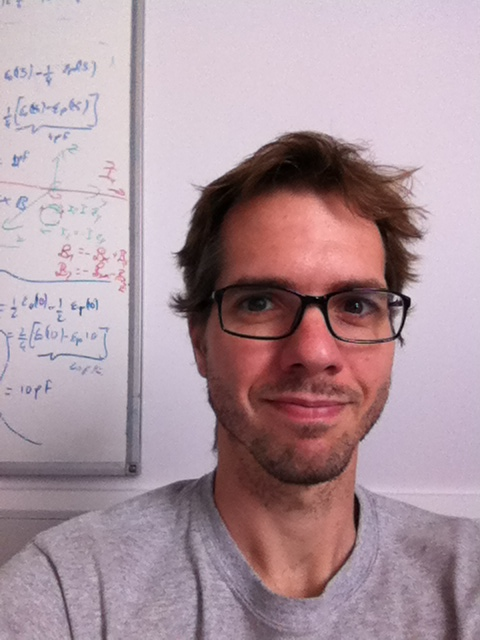
\includegraphics[width=1in,height=1.25in,clip,keepaspectratio]{images/JAV-Website-Photo.jpg}}]{Javier Alonso-Valdesueiro} was born in Madrid, Spain, in 1980. He received his Telecommunications Engineering degree from the University of Alcalá, Madrid, in 2006, and his Ph.D. degree from the Polytechnic University of Catalonia, Barcelona, in 2011. From 2012 to 2020, he worked on developing electronic instrumentation for NMR experiments, initially at the C.E.A Center in France, followed by the University of Southampton in the UK, and later as a Marie Skłodowska-Curie Fellow at the University of the Basque Country (UPV/EHU). Over the past four years, he has advanced his career as an RF and instrumentation engineer in both private companies and public research centers, including TECNALIA Innovation Foundation and the Institute of Biomedical Engineering of Catalonia. Recently, he has been appointed as Assistant Professor in the Department of Electronic and Biomedical Engineering at the University of Barcelona.
\end{IEEEbiography}
\vskip -2\baselineskip plus -1fil
\vfill

\end{document}


